\documentclass[11pt]{article}

\usepackage[margin=1in]{geometry}
\usepackage[T1]{fontenc}
\usepackage[utf8]{inputenc}
\usepackage{lmodern}
\usepackage{microtype}
\usepackage{amsmath,amssymb,mathtools,bm}
\usepackage{booktabs,array,longtable}
\usepackage{hyperref}
\usepackage{xcolor}
\usepackage[most]{tcolorbox}
\usepackage{tikz}
\usepackage{pgfplots}
\usepackage{tikz-3dplot}
\usepackage{enumitem}
\usepackage{caption}
\usepackage{float}
\usepackage{fancyhdr}
\usepackage{titlesec}

\pgfplotsset{compat=1.18}
\usetikzlibrary{arrows.meta,calc,patterns,positioning,decorations.pathreplacing,backgrounds,3d}

\hypersetup{
  colorlinks=true,
  linkcolor=blue!60!black,
  urlcolor=blue!60!black,
  citecolor=blue!60!black,
  pdftitle={Chapter 11. Directional Derivatives, Hessians, and Optimization}
}

\setlength{\headheight}{14pt}
\setlength{\parindent}{0pt}
\setlength{\parskip}{0.65em}
\setlist[itemize]{topsep=2pt,itemsep=2pt}
\setlist[enumerate]{topsep=2pt,itemsep=2pt}

\titleformat{\section}{\large\bfseries}{\thesection}{0.6em}{}
\titleformat{\subsection}{\normalsize\bfseries}{\thesubsection}{0.6em}{}

\pagestyle{fancy}
\fancyhf{}
\lhead{Chapter 11. Directional Derivatives, Hessians, and Optimization}
\rhead{\thepage}
\renewcommand{\headrulewidth}{0.4pt}

\newtcolorbox{chaptergoalbox}{
  colback=blue!4,
  colframe=blue!55!black,
  boxrule=0.7pt,
  arc=2mm,
  left=2mm,right=2mm,top=1mm,bottom=1mm
}
\newtcolorbox{goalbox}{
  colback=green!4,
  colframe=green!45!black,
  title=Learning objectives,
  fonttitle=\bfseries,
  boxrule=0.7pt,
  arc=2mm
}
\newtcolorbox{notebox}[1][]{
  colback=blue!3,
  colframe=blue!50!black,
  fonttitle=\bfseries,
  title=#1,
  boxrule=0.7pt,
  arc=2mm
}
\newtcolorbox{importantbox}[1][]{
  colback=red!3,
  colframe=red!60!black,
  fonttitle=\bfseries,
  title=#1,
  boxrule=0.7pt,
  arc=2mm
}
\newtcolorbox{tipbox}[1][]{
  colback=green!3,
  colframe=green!45!black,
  fonttitle=\bfseries,
  title=#1,
  boxrule=0.7pt,
  arc=2mm
}
\newtcolorbox{warningbox}[1][]{
  colback=yellow!8,
  colframe=orange!75!black,
  fonttitle=\bfseries,
  title=#1,
  boxrule=0.7pt,
  arc=2mm
}
\newtcbtheorem[number within=section]{workedexample}{Worked example}{
  enhanced,
  breakable,
  colback=white,
  colframe=blue!60!black,
  colbacktitle=blue!60!black,
  fonttitle=\bfseries,
  boxrule=0.7pt,
  arc=1.5mm,
  left=2mm,right=2mm,top=1mm,bottom=1mm
}{ex}

\newcommand{\R}{\mathbb R}
\newcommand{\grad}{\nabla}
\newcommand{\norm}[1]{\left\lVert #1\right\rVert}
\newcommand{\bmat}[1]{\begin{bmatrix}#1\end{bmatrix}}

\begin{document}

\begin{center}
  {\LARGE\bfseries Chapter 11. Directional Derivatives, Hessians, and Optimization\par}
  \vspace{0.3em}
  {\large From local rates of change to modern loss landscapes\par}
\end{center}

\begin{chaptergoalbox}
\textbf{Chapter goal.} In this chapter we turn derivatives into decisions. A gradient tells us how a function changes when we move in a chosen direction. A Hessian tells us the local curvature of a surface or a loss function. Together, they give a practical language for maxima, minima, saddle points, and numerical optimization.

A function of one variable has only two local directions: left and right. A function of two or more variables has infinitely many directions. At a point on a surface $z=f(x,y)$, we can move east, west, north, south, northeast, or along any unit direction $u$. The \emph{directional derivative} measures the rate of change in that direction.
\end{chaptergoalbox}

This idea is central in applied mathematics, statistics, data science, and machine learning. A statistical loss function or negative log-likelihood is usually a function of many parameters. To minimize it, we must know which direction decreases the loss most rapidly. The answer is built from the gradient and refined by the Hessian.

\begin{goalbox}
After studying this chapter, you should be able to:
\begin{enumerate}
  \item compute directional derivatives using the formula $D_u f=\grad f\cdot u$;
  \item explain why the gradient points in the direction of steepest increase;
  \item find and classify critical points of functions of two variables;
  \item use the Hessian matrix and the second derivative test;
  \item distinguish local extrema, absolute extrema, and saddle points;
  \item solve absolute optimization problems on closed bounded regions;
  \item implement gradient descent and Newton's method for two-variable functions;
  \item interpret optimization as the geometric core of modern model fitting.
\end{enumerate}
\end{goalbox}

\section{Directional derivatives}

Let $f(x,y)$ be a differentiable function and let $u=\langle a,b\rangle$ be a unit vector. The \emph{directional derivative} of $f$ at $(x_0,y_0)$ in the direction $u$ is
\[
D_u f(x_0,y_0)=\lim_{h\to 0}\frac{f(x_0+ha,y_0+hb)-f(x_0,y_0)}{h}.
\]
This is the rate of change of $f$ as we move from $(x_0,y_0)$ in the direction $u$.

The important computational formula is
\[
D_u f(x,y)=\grad f(x,y)\cdot u.
\]
For a function of three variables, if $u=\langle a,b,c\rangle$ is a unit vector, then
\[
D_u f(x,y,z)=\grad f(x,y,z)\cdot u.
\]

\begin{notebox}[Always normalize the direction vector]
The direction vector in a directional derivative must be a \emph{unit vector}. If the problem gives a nonzero vector $v$, first compute
\[
u=\frac{v}{\norm{v}}.
\]
Then use $D_u f=\grad f\cdot u$.
\end{notebox}

\begin{workedexample}{A directional derivative from a non-unit vector}{dir-nonunit}
Let
\[
f(x,y)=x^2+3xy-2y^4.
\]
Find $D_u f(0,1)$ in the direction of $v=\langle 1,2\rangle$.

First compute the gradient:
\[
\grad f(x,y)=\langle 2x+3y,3x-8y^3\rangle.
\]
At $(0,1)$,
\[
\grad f(0,1)=\langle 3,-8\rangle.
\]
The vector $v=\langle 1,2\rangle$ has length $\sqrt5$, so
\[
u=\frac{1}{\sqrt5}\langle 1,2\rangle.
\]
Therefore
\[
D_u f(0,1)=\langle 3,-8\rangle\cdot \left\langle \frac{1}{\sqrt5},\frac{2}{\sqrt5}\right\rangle
=\frac{3-16}{\sqrt5}=-\frac{13}{\sqrt5}.
\]
The negative sign means that $f$ is decreasing in the direction $\langle 1,2\rangle$ at $(0,1)$.
\end{workedexample}

\begin{figure}[H]
\centering
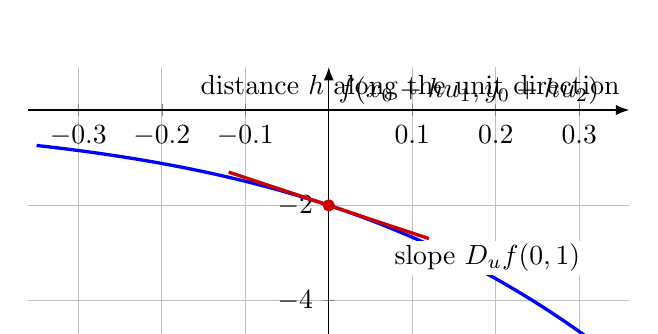
\begin{tikzpicture}
\begin{axis}[
  width=0.76\textwidth,
  height=0.42\textwidth,
  xlabel={distance $h$ along the unit direction},
  ylabel={$f(x_0+h u_1,y_0+h u_2)$},
  xmin=-0.36,xmax=0.36,
  ymin=-4.9,ymax=0.9,
  grid=both,
  axis lines=middle,
  axis line style={-Latex},
  samples=240,
]
\addplot[very thick,blue,domain=-0.35:0.35] {((x/sqrt(5))^2 + 3*(x/sqrt(5))*(1+2*x/sqrt(5)) - 2*(1+2*x/sqrt(5))^4)};
\addplot[only marks,mark=*,mark size=2pt,red!80!black] coordinates {(0,-2)};
\addplot[red!80!black,very thick,domain=-0.12:0.12] {-2 - 13/sqrt(5)*x};
\node[fill=white,inner sep=1.2pt] at (axis cs:0.19,-3.1) {slope $D_u f(0,1)$};
\end{axis}
\end{tikzpicture}
\caption{A directional derivative is the slope of a one-variable slice through a surface.}
\end{figure}

\section{The gradient as the direction of steepest increase}

The formula $D_u f=\grad f\cdot u$ has a powerful geometric interpretation. If $u$ is a unit vector, then
\[
D_u f=\grad f\cdot u=\norm{\grad f}\norm{u}\cos\theta=\norm{\grad f}\cos\theta,
\]
where $\theta$ is the angle between $\grad f$ and $u$. Since $-1\le \cos\theta\le 1$,
\[
-\norm{\grad f}\le D_u f\le \norm{\grad f}.
\]
Thus the maximum directional derivative is $\norm{\grad f}$, attained in the direction of $\grad f$, and the minimum directional derivative is $-\norm{\grad f}$, attained in the opposite direction.

\begin{importantbox}[Steepest directions]
At a point where $\grad f\ne 0$,
\[
\text{steepest ascent direction}=\frac{\grad f}{\norm{\grad f}},
\qquad
\text{steepest descent direction}=-\frac{\grad f}{\norm{\grad f}}.
\]
\end{importantbox}

This is the geometric reason gradient descent works: to decrease a differentiable function rapidly, move approximately in the direction $-\grad f$.

\begin{workedexample}{Fastest increase of temperature}{temperature}
Suppose the temperature at a point $(x,y,z)$ is
\[
T(x,y,z)=xe^y+\frac12 z^2.
\]
The gradient is
\[
\grad T(x,y,z)=\langle e^y,xe^y,z\rangle.
\]
At $(1,0,3)$,
\[
\grad T(1,0,3)=\langle 1,1,3\rangle.
\]
Therefore the direction of fastest increase is
\[
\frac{1}{\sqrt{11}}\langle 1,1,3\rangle,
\]
and the maximum rate of increase is $\norm{\grad T(1,0,3)}=\sqrt{11}$.
\end{workedexample}

\begin{workedexample}{Climbing a hill}{hill}
Suppose a hill is modeled by
\[
z=f(x,y)=1100-2x^2-y^2,
\]
where $x$ and $y$ are measured in meters. At $(10,20)$,
\[
\grad f(x,y)=\langle -4x,-2y\rangle,
\qquad
\grad f(10,20)=\langle -40,-40\rangle.
\]
The hill rises fastest in the southwest direction
\[
\frac{1}{\sqrt2}\langle -1,-1\rangle,
\]
and the maximum rate of increase is $40\sqrt2$.
\end{workedexample}

\begin{figure}[H]
\centering
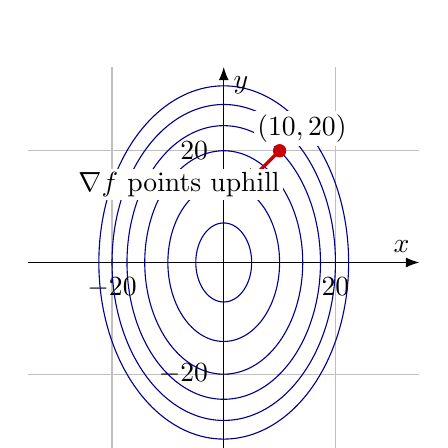
\begin{tikzpicture}
\begin{axis}[
  width=0.68\textwidth,
  height=0.54\textwidth,
  xmin=-35,xmax=35,
  ymin=-35,ymax=35,
  axis equal image,
  axis lines=middle,
  xlabel={$x$},ylabel={$y$},
  grid=both,
  axis line style={-Latex},
]
\foreach \c in {100,300,500,700,900,1050}{
  \pgfmathsetmacro{\rx}{sqrt((1100-\c)/2)}
  \pgfmathsetmacro{\ry}{sqrt(1100-\c)}
  \addplot[domain=0:360,samples=180,blue!55!black] ({\rx*cos(x)},{\ry*sin(x)});
}
\addplot[only marks,mark=*,mark size=2.2pt,red!80!black] coordinates {(10,20)};
\addplot[red!80!black,very thick,-Latex] coordinates {(10,20) (2.9,12.9)};
\node[fill=white,inner sep=1.2pt] at (axis cs:14,24) {$(10,20)$};
\node[fill=white,inner sep=1.2pt] at (axis cs:-8,14) {$\grad f$ points uphill};
\end{axis}
\end{tikzpicture}
\caption{The gradient on a contour map points in the direction of fastest increase.}
\end{figure}

\section{Gradients and level curves}

A level curve of $f$ is a curve $f(x,y)=c$. If a differentiable curve $r(t)=\langle x(t),y(t)\rangle$ stays on the level curve, then $f(x(t),y(t))=c$. Differentiating gives
\[
\grad f(x(t),y(t))\cdot r'(t)=0.
\]
So the gradient is perpendicular to the tangent vector of the level curve.

\begin{notebox}[Gradient and level curves]
At a regular point of a level curve, $\grad f$ is normal to the level curve. Closely spaced level curves usually indicate a large gradient magnitude.
\end{notebox}

\begin{figure}[H]
\centering
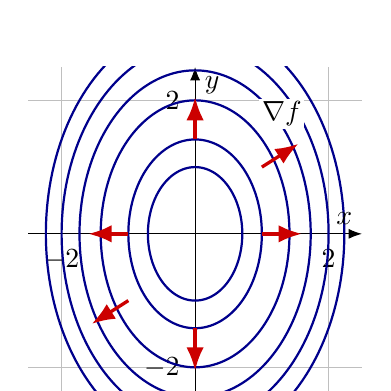
\begin{tikzpicture}
\begin{axis}[
  width=0.66\textwidth,
  height=0.48\textwidth,
  xmin=-2.5,xmax=2.5,
  ymin=-2.5,ymax=2.5,
  axis equal image,
  axis lines=middle,
  xlabel={$x$},ylabel={$y$},
  grid=both,
  axis line style={-Latex},
]
\foreach \c in {0.5,1,2,3,4,5}{
  \addplot[domain=0:360,samples=180,blue!55!black,thick] ({sqrt(\c)*cos(x)},{sqrt(2*\c)*sin(x)});
}
\foreach \px/\py/\qx/\qy in {1/0/1.6/0,0/1.414/0/2.05,-1/0/-1.6/0,0/-1.414/0/-2.05,1/1/1.55/1.35,-1/-1/-1.55/-1.35}{
  \addplot[red!80!black,very thick,-Latex] coordinates {(\px,\py) (\qx,\qy)};
}
\node[fill=white,inner sep=1pt] at (axis cs:1.3,1.8) {$\grad f$};
\end{axis}
\end{tikzpicture}
\caption{Gradient vectors are perpendicular to level curves and point toward increasing values.}
\end{figure}

\section{Critical points and local extrema}

A function $f(x,y)$ has a \emph{local maximum} at $(a,b)$ if $f(x,y)\le f(a,b)$ for all points sufficiently close to $(a,b)$. It has a \emph{local minimum} at $(a,b)$ if $f(x,y)\ge f(a,b)$ for all points sufficiently close to $(a,b)$.

A point $(a,b)$ is called a \emph{critical point} if
\[
\grad f(a,b)=0,
\]
or if one of the first partial derivatives fails to exist.

\begin{importantbox}[First derivative test for possible extrema]
If $f$ has a local maximum or local minimum at $(a,b)$ and the first partial derivatives exist there, then
\[
f_x(a,b)=0,\qquad f_y(a,b)=0.
\]
So local extrema can occur only at critical points, boundary points, or points where differentiability fails.
\end{importantbox}

\begin{workedexample}{A quadratic local minimum}{quad-min}
Let
\[
f(x,y)=x^2+y^2-4x-2y+18.
\]
The gradient is
\[
\grad f(x,y)=\langle 2x-4,2y-2\rangle.
\]
Setting $\grad f=0$ gives $x=2$ and $y=1$. Completing the square,
\[
f(x,y)=(x-2)^2+(y-1)^2+13.
\]
So $f$ has a local and absolute minimum at $(2,1)$, with minimum value $13$.
\end{workedexample}

\begin{workedexample}{A saddle point}{saddle}
Let $f(x,y)=y^2-x^2$. Then
\[
\grad f(x,y)=\langle -2x,2y\rangle,
\]
so the only critical point is $(0,0)$. Along the $y$-axis, $f(0,y)=y^2\ge 0$, while along the $x$-axis, $f(x,0)=-x^2\le 0$. Thus $(0,0)$ is neither a local maximum nor a local minimum. It is a \emph{saddle point}.
\end{workedexample}

\begin{figure}[H]
\centering
\begin{minipage}{0.48\textwidth}
\centering
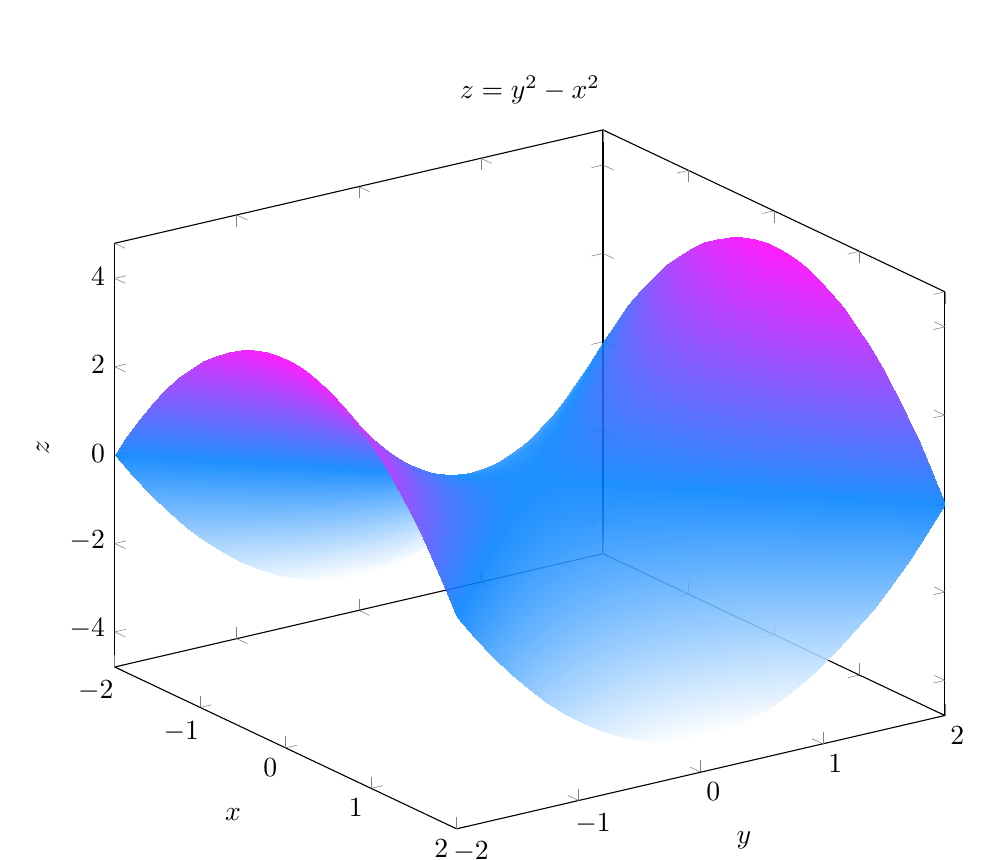
\begin{tikzpicture}
\begin{axis}[
  width=\textwidth,
  view={55}{25},
  xlabel={$x$},ylabel={$y$},zlabel={$z$},
  domain=-2:2, y domain=-2:2,
  samples=28,samples y=28,
  colormap/cool,
  title={$z=y^2-x^2$},
]
\addplot3[surf,shader=interp,opacity=0.88] {y^2-x^2};
\end{axis}
\end{tikzpicture}
\end{minipage}\hfill
\begin{minipage}{0.48\textwidth}
\centering
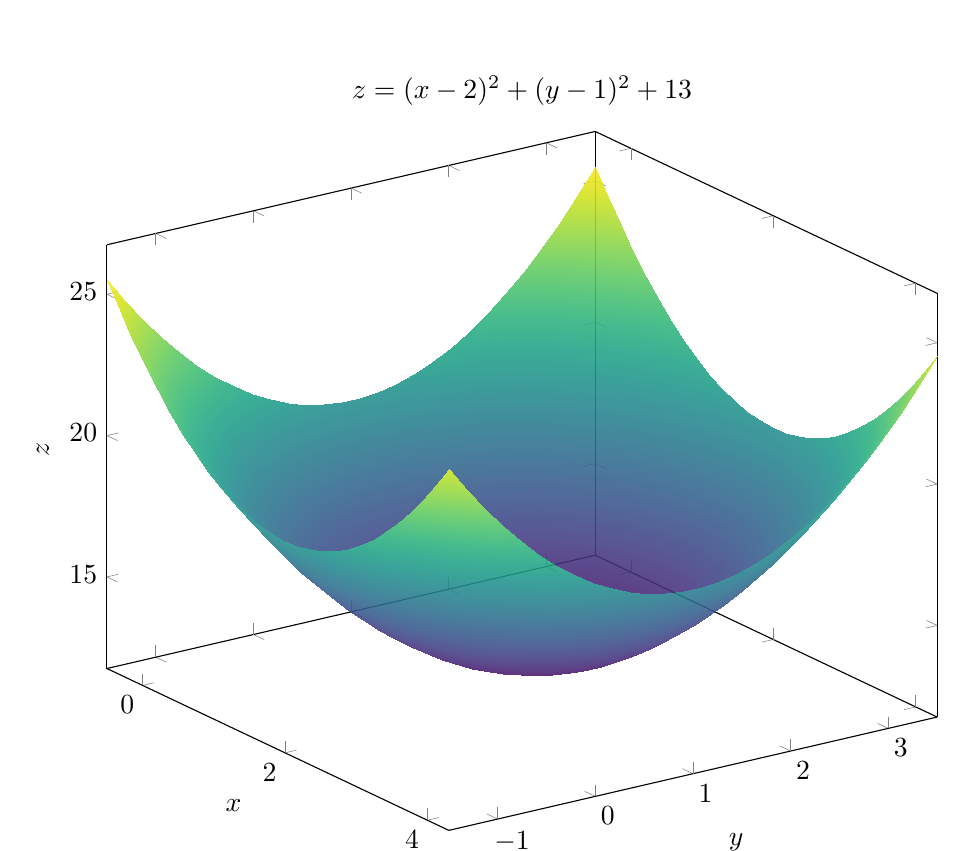
\begin{tikzpicture}
\begin{axis}[
  width=\textwidth,
  view={55}{25},
  xlabel={$x$},ylabel={$y$},zlabel={$z$},
  domain=-0.5:4.3, y domain=-1.5:3.5,
  samples=28,samples y=28,
  colormap/viridis,
  title={$z=(x-2)^2+(y-1)^2+13$},
]
\addplot3[surf,shader=interp,opacity=0.88] {(x-2)^2+(y-1)^2+13};
\end{axis}
\end{tikzpicture}
\end{minipage}
\caption{A saddle point has mixed curvature, while a local minimum curves upward in all directions.}
\end{figure}

\section{The Hessian matrix and second derivative test}

The second derivative information of a function $f(x,y)$ is organized into the \emph{Hessian matrix}
\[
H_f(x,y)=\bmat{f_{xx}(x,y)&f_{xy}(x,y)\\ f_{yx}(x,y)&f_{yy}(x,y)}.
\]
When $f_{xy}=f_{yx}$, this matrix is symmetric. Near a critical point $(a,b)$, the quadratic part of the Taylor approximation is
\[
\frac12\bmat{x-a&y-b}H_f(a,b)\bmat{x-a\\y-b}.
\]
So the Hessian describes local curvature.

For two-variable functions, define
\[
D(a,b)=f_{xx}(a,b)f_{yy}(a,b)-[f_{xy}(a,b)]^2.
\]
This is the determinant of the Hessian matrix.

\begin{tipbox}[Second derivative test]
Suppose $f_x(a,b)=0$, $f_y(a,b)=0$, and the second partial derivatives are continuous near $(a,b)$.
\begin{itemize}
  \item If $D(a,b)>0$ and $f_{xx}(a,b)>0$, then $f$ has a local minimum at $(a,b)$.
  \item If $D(a,b)>0$ and $f_{xx}(a,b)<0$, then $f$ has a local maximum at $(a,b)$.
  \item If $D(a,b)<0$, then $f$ has a saddle point at $(a,b)$.
  \item If $D(a,b)=0$, the test is inconclusive.
\end{itemize}
\end{tipbox}

The determinant works because the Hessian represents the local quadratic shape. Positive curvature in all directions gives a local minimum, negative curvature in all directions gives a local maximum, and mixed signs give a saddle. This is the two-dimensional version of the eigenvalue test for quadratic forms.

\begin{workedexample}{Classifying critical points}{classify-cubic}
Let
\[
f(x,y)=x^3+y^3-3xy+4.
\]
The first derivatives are
\[
f_x=3x^2-3y,\qquad f_y=3y^2-3x.
\]
Setting them equal to zero gives $y=x^2$ and $x=y^2$. Hence $x=x^4$, so $x=0$ or $x=1$. The critical points are $(0,0)$ and $(1,1)$.

The second derivatives are
\[
f_{xx}=6x,\qquad f_{yy}=6y,\qquad f_{xy}=-3.
\]
Thus $D(x,y)=36xy-9$. At $(0,0)$, $D=-9<0$, so $(0,0)$ is a saddle point. At $(1,1)$, $D=27>0$ and $f_{xx}=6>0$, so $(1,1)$ is a local minimum. The minimum value is $f(1,1)=3$.
\end{workedexample}

\begin{figure}[H]
\centering
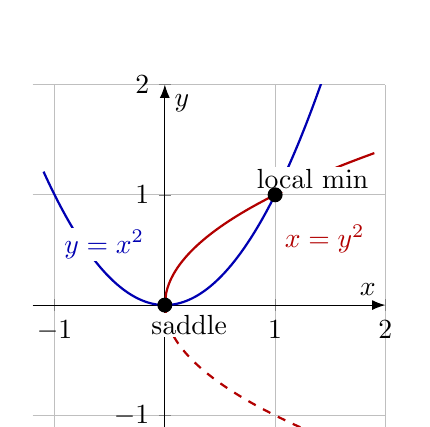
\begin{tikzpicture}
\begin{axis}[
  width=0.68\textwidth,
  height=0.50\textwidth,
  xmin=-1.2,xmax=2.0,
  ymin=-1.2,ymax=2.0,
  axis equal image,
  axis lines=middle,
  xlabel={$x$},ylabel={$y$},
  grid=both,
  axis line style={-Latex},
]
\addplot[domain=-1.1:1.55,samples=160,blue!70!black,thick] {x^2};
\addplot[domain=0:1.9,samples=160,red!70!black,thick] {sqrt(x)};
\addplot[domain=0:1.9,samples=160,red!70!black,thick,dashed] {-sqrt(x)};
\addplot[only marks,mark=*,mark size=2.5pt] coordinates {(0,0) (1,1)};
\node[fill=white,inner sep=1pt] at (axis cs:0.22,-0.18) {saddle};
\node[fill=white,inner sep=1pt] at (axis cs:1.34,1.14) {local min};
\node[blue!70!black,fill=white,inner sep=1pt] at (axis cs:-0.55,0.55) {$y=x^2$};
\node[red!70!black,fill=white,inner sep=1pt] at (axis cs:1.45,0.6) {$x=y^2$};
\end{axis}
\end{tikzpicture}
\caption{Critical points of $x^3+y^3-3xy+4$ occur where $y=x^2$ and $x=y^2$ intersect.}
\end{figure}

\begin{workedexample}{Four critical points}{fourcrit}
Let
\[
f(x,y)=x^3+y^3+3x^2-3y^2-7.
\]
The first derivatives are $f_x=3x(x+2)$ and $f_y=3y(y-2)$. Therefore
\[
x=0\text{ or }x=-2,
\qquad
 y=0\text{ or }y=2.
\]
The critical points are $(0,0)$, $(0,2)$, $(-2,0)$, and $(-2,2)$. Since $f_{xx}=6x+6$, $f_{yy}=6y-6$, and $f_{xy}=0$, the determinant is $D=f_{xx}f_{yy}$.
\begin{itemize}
  \item $(0,0)$: $D=6(-6)<0$, saddle point.
  \item $(0,2)$: $D=6(6)>0$ and $f_{xx}>0$, local minimum.
  \item $(-2,0)$: $D=(-6)(-6)>0$ and $f_{xx}<0$, local maximum.
  \item $(-2,2)$: $D=(-6)(6)<0$, saddle point.
\end{itemize}
\end{workedexample}

\section{Absolute extrema on closed bounded regions}

Local extrema describe what happens near a point. Absolute extrema describe the largest and smallest values on an entire region.

\begin{notebox}[Extreme value principle]
If $f$ is continuous on a closed and bounded region $D\subset \R^2$, then $f$ attains both an absolute maximum and an absolute minimum on $D$.
\end{notebox}

To find absolute extrema on a closed bounded region:
\begin{enumerate}
  \item find critical points inside $D$;
  \item find extrema on the boundary of $D$;
  \item compare all candidate values.
\end{enumerate}

\begin{workedexample}{Extrema on a rectangle}{rect-extrema}
Find the absolute maximum and minimum of
\[
f(x,y)=x^2-2xy+2y
\]
on the rectangle $0\le x\le 3$, $0\le y\le 2$.

Interior critical points satisfy
\[
f_x=2x-2y=0,\qquad f_y=-2x+2=0,
\]
so $x=1$ and $y=1$. The interior value is $f(1,1)=1$.

On the four boundary sides:
\[
x=0:\ f=2y,
\qquad
x=3:\ f=9-4y,
\]
\[
y=0:\ f=x^2,
\qquad
y=2:\ f=(x-2)^2.
\]
Comparing all candidates, the absolute maximum value is $9$, attained at $(3,0)$, and the absolute minimum value is $0$, attained at $(0,0)$ and $(2,2)$.
\end{workedexample}

\begin{figure}[H]
\centering
\begin{minipage}{0.48\textwidth}
\centering
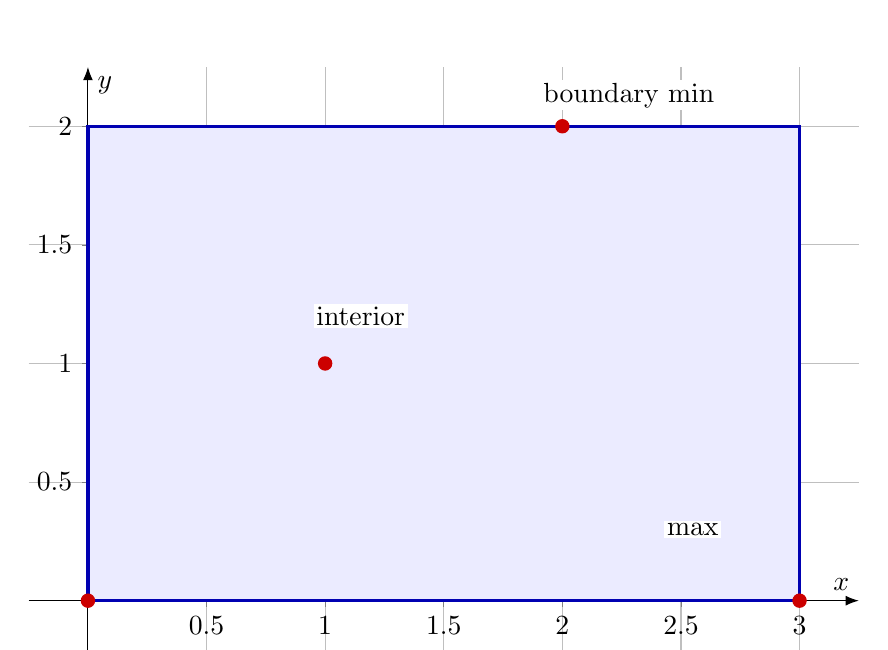
\begin{tikzpicture}
\begin{axis}[
  width=\textwidth,
  height=0.78\textwidth,
  xmin=-0.25,xmax=3.25,
  ymin=-0.25,ymax=2.25,
  axis equal image,
  axis lines=middle,
  xlabel={$x$},ylabel={$y$},
  grid=both,
  axis line style={-Latex},
]
\draw[fill=blue!8,draw=blue!70!black,very thick] (axis cs:0,0) rectangle (axis cs:3,2);
\addplot[only marks,mark=*,mark size=2.4pt,red!80!black] coordinates {(1,1) (3,0) (0,0) (2,2)};
\node[fill=white,inner sep=1pt] at (axis cs:1.15,1.2) {interior};
\node[fill=white,inner sep=1pt] at (axis cs:2.28,2.13) {boundary min};
\node[fill=white,inner sep=1pt] at (axis cs:2.55,0.3) {max};
\end{axis}
\end{tikzpicture}
\caption*{Rectangle: compare interior and boundary candidates.}
\end{minipage}\hfill
\begin{minipage}{0.48\textwidth}
\centering
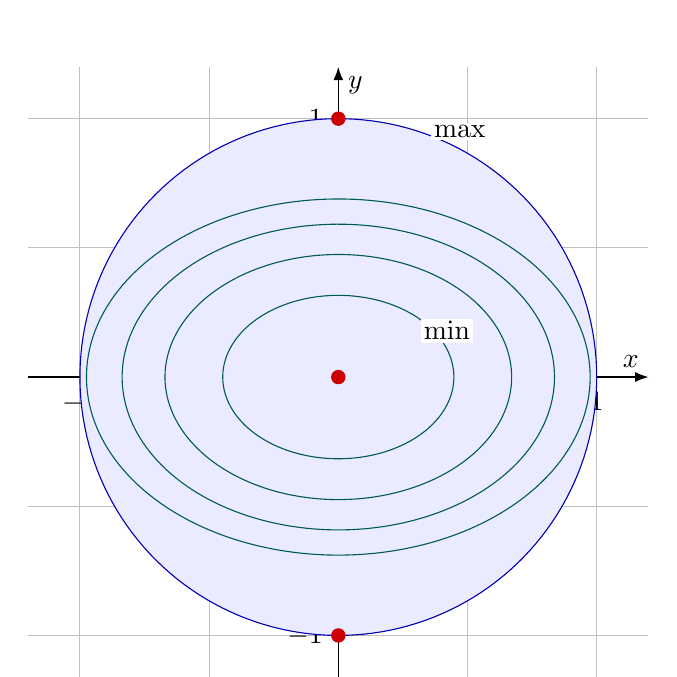
\begin{tikzpicture}
\begin{axis}[
  width=\textwidth,
  height=0.78\textwidth,
  xmin=-1.2,xmax=1.2,
  ymin=-1.2,ymax=1.2,
  axis equal image,
  axis lines=middle,
  xlabel={$x$},ylabel={$y$},
  grid=both,
  axis line style={-Latex},
]
\addplot[draw=blue!70!black,fill=blue!8,domain=0:360,samples=180] ({cos(x)},{sin(x)}) -- cycle;
\foreach \c in {0.2,0.45,0.7,0.95}{
  \addplot[domain=0:360,samples=180,teal!70!black] ({sqrt(\c)*cos(x)},{sqrt(\c/2)*sin(x)});
}
\addplot[only marks,mark=*,mark size=2.4pt,red!80!black] coordinates {(0,0) (0,1) (0,-1)};
\node[fill=white,inner sep=1pt] at (axis cs:0.42,0.18) {min};
\node[fill=white,inner sep=1pt] at (axis cs:0.47,0.95) {max};
\end{axis}
\end{tikzpicture}
\caption*{Disk: check the center and the boundary circle.}
\end{minipage}
\caption{Absolute extrema on closed bounded regions require checking both interior critical points and boundary candidates.}
\end{figure}

\begin{workedexample}{Extrema on a disk}{disk-extrema}
Find the extreme values of
\[
f(x,y)=x^2+2y^2+2
\]
on the disk $x^2+y^2\le 1$. The gradient is $\grad f=\langle 2x,4y\rangle$, so the only interior critical point is $(0,0)$, where $f(0,0)=2$.

On the boundary $x^2+y^2=1$,
\[
f(x,y)=x^2+2y^2+2=(1-y^2)+2y^2+2=3+y^2.
\]
Since $0\le y^2\le 1$, the boundary values satisfy $3\le f\le 4$. Therefore the absolute minimum is $2$ at $(0,0)$, and the absolute maximum is $4$ at $(0,1)$ and $(0,-1)$.
\end{workedexample}

\section{Gradient descent}

Many optimization problems in statistics and machine learning cannot be solved exactly by hand. Instead, we use iterative algorithms. The most basic method is \emph{gradient descent}. To minimize a differentiable function $L(\theta)$, start with an initial guess $\theta_0$ and update by
\[
\theta_{k+1}=\theta_k-\eta\grad L(\theta_k),
\]
where $\eta>0$ is the learning rate.

The idea is simple: $\grad L$ points in the direction of steepest increase, so $-\grad L$ points in the direction of steepest decrease. The learning rate controls the step size.

\begin{workedexample}{Gradient descent on a quadratic loss}{gd-quad}
Consider
\[
L(x,y)=3(x-1)^2+(y+2)^2+xy.
\]
The gradient is
\[
\grad L(x,y)=\langle 6(x-1)+y,2(y+2)+x\rangle.
\]
The critical point solves
\[
6(x-1)+y=0,
\qquad
2(y+2)+x=0.
\]
Solving gives
\[
(x,y)=\left(\frac{16}{11},-\frac{30}{11}\right).
\]
Gradient descent approaches this point when the learning rate is chosen appropriately.
\end{workedexample}

\begin{figure}[H]
\centering
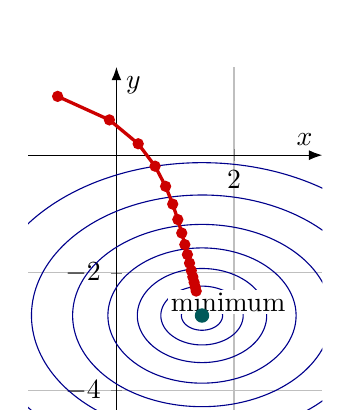
\begin{tikzpicture}
\begin{axis}[
  width=0.72\textwidth,
  height=0.50\textwidth,
  xmin=-1.5,xmax=3.5,
  ymin=-4.5,ymax=1.5,
  axis equal image,
  axis lines=middle,
  xlabel={$x$},ylabel={$y$},
  grid=both,
  axis line style={-Latex},
]
\foreach \a/\b in {0.35/0.25,0.7/0.5,1.1/0.8,1.6/1.15,2.2/1.55,2.9/2.05,3.7/2.6}{
  \addplot[domain=0:360,samples=180,blue!55!black] ({1.455 + \a*cos(x)},{-2.727 + \b*sin(x)});
}
\addplot[red!80!black,very thick,mark=*,mark size=1.4pt] coordinates {(-1.000,1.000) (-0.120,0.600) (0.370,0.194) (0.657,-0.187) (0.836,-0.530) (0.957,-0.832) (1.044,-1.095) (1.111,-1.324) (1.163,-1.521) (1.207,-1.690) (1.243,-1.836) (1.273,-1.962) (1.299,-2.070) (1.321,-2.163) (1.340,-2.242) (1.356,-2.311)};
\addplot[only marks,mark=*,mark size=2.4pt,teal!70!black] coordinates {(1.455,-2.727)};
\node[fill=white,inner sep=1pt] at (axis cs:1.9,-2.5) {minimum};
\end{axis}
\end{tikzpicture}
\caption{Gradient descent follows the negative gradient direction toward a local minimum.}
\end{figure}

\section{Least squares as an optimization problem}

Suppose we have data points $(x_i,y_i)$ and model them with a line
\[
\hat y_i=\beta_0+\beta_1x_i.
\]
The least-squares loss is
\[
L(\beta_0,\beta_1)=\sum_{i=1}^n \left[y_i-(\beta_0+\beta_1x_i)\right]^2.
\]
This is a function of two variables: the intercept $\beta_0$ and the slope $\beta_1$. The best-fit line is the point in parameter space where this loss is minimized.

The gradient is
\[
\frac{\partial L}{\partial \beta_0}=-2\sum_{i=1}^n \left[y_i-(\beta_0+\beta_1x_i)\right],
\]
and
\[
\frac{\partial L}{\partial \beta_1}=-2\sum_{i=1}^n x_i\left[y_i-(\beta_0+\beta_1x_i)\right].
\]
Gradient descent updates the parameters by moving opposite this gradient.

\begin{figure}[H]
\centering
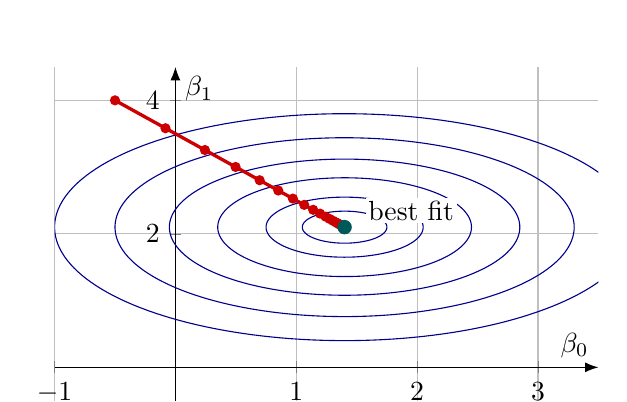
\begin{tikzpicture}
\begin{axis}[
  width=0.70\textwidth,
  height=0.48\textwidth,
  xmin=-1,xmax=3.5,
  ymin=-0.5,ymax=4.5,
  axis lines=middle,
  xlabel={$\beta_0$},ylabel={$\beta_1$},
  grid=both,
  axis line style={-Latex},
]
\foreach \a/\b in {0.35/0.24,0.65/0.45,1.05/0.74,1.45/1.02,1.9/1.34,2.4/1.7}{
  \addplot[domain=0:360,samples=180,blue!55!black] ({1.4 + \a*cos(x)},{2.1 + \b*sin(x)});
}
\addplot[red!80!black,very thick,mark=*,mark size=1.2pt] coordinates {(-0.500,4.000) (-0.082,3.582) (0.244,3.256) (0.498,3.002) (0.697,2.803) (0.851,2.649) (0.972,2.528) (1.066,2.434) (1.140,2.360) (1.197,2.303) (1.242,2.258) (1.276,2.224) (1.304,2.196) (1.325,2.175) (1.341,2.159) (1.354,2.146) (1.364,2.136) (1.372,2.128)};
\addplot[only marks,mark=*,mark size=2.4pt,teal!70!black] coordinates {(1.4,2.1)};
\node[fill=white,inner sep=1pt] at (axis cs:1.95,2.35) {best fit};
\end{axis}
\end{tikzpicture}
\caption{Least-squares fitting minimizes a loss function over parameter space.}
\end{figure}

\section{Newton's method in several variables}

Gradient descent uses first derivative information. Newton's method also uses second derivative information. For a function $L(\theta)$ with gradient $\grad L(\theta)$ and Hessian $H_L(\theta)$, Newton's update is
\[
\theta_{k+1}=\theta_k-H_L(\theta_k)^{-1}\grad L(\theta_k).
\]
Equivalently, solve the linear system
\[
H_L(\theta_k)s_k=-\grad L(\theta_k)
\]
and set $\theta_{k+1}=\theta_k+s_k$.

Newton's method can be very fast near a local minimum when the Hessian is positive definite. However, it can behave poorly near saddle points or when the Hessian is singular or indefinite. In large-scale machine learning, full Newton steps may be too expensive, so many algorithms use approximations to Hessian information.

\begin{figure}[H]
\centering
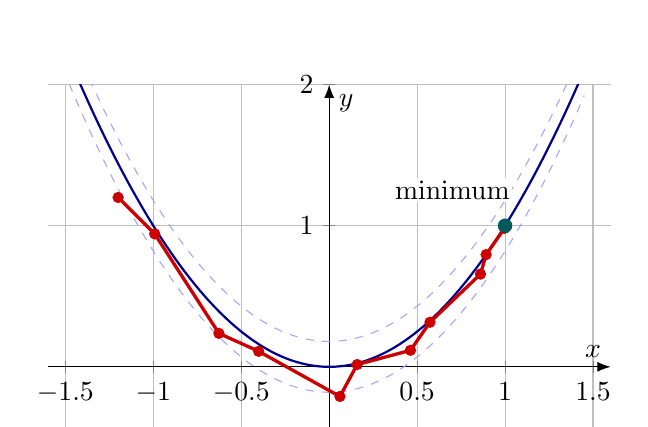
\begin{tikzpicture}
\begin{axis}[
  width=0.72\textwidth,
  height=0.50\textwidth,
  xmin=-1.6,xmax=1.6,
  ymin=-0.5,ymax=2.0,
  axis lines=middle,
  xlabel={$x$},ylabel={$y$},
  grid=both,
  axis line style={-Latex},
]
\addplot[domain=-1.55:1.45,samples=200,blue!55!black,thick] {x^2};
\addplot[domain=-1.55:1.45,samples=200,blue!35,dashed] {x^2+0.18};
\addplot[domain=-1.55:1.45,samples=200,blue!35,dashed] {x^2-0.18};
\addplot[red!80!black,very thick,mark=*,mark size=1.4pt] coordinates {(-1.200,1.200) (-0.992,0.942) (-0.627,0.237) (-0.401,0.110) (0.061,-0.210) (0.159,0.016) (0.462,0.117) (0.573,0.316) (0.860,0.657) (0.892,0.795) (0.996,0.981)};
\addplot[only marks,mark=*,mark size=2.4pt,teal!70!black] coordinates {(1,1)};
\node[fill=white,inner sep=1pt] at (axis cs:0.7,1.25) {minimum};
\end{axis}
\end{tikzpicture}
\caption{Newton-type steps use curvature information and can move differently from gradient descent.}
\end{figure}

\section{Practical optimization workflow}

For a smooth function $L(\theta)$, a standard optimization workflow is:
\begin{enumerate}
  \item \textbf{Model the objective.} Decide what function should be minimized or maximized.
  \item \textbf{Compute the gradient.} Use calculus, automatic differentiation, or finite differences.
  \item \textbf{Find critical points.} Solve $\grad L=0$ when possible.
  \item \textbf{Use the Hessian.} Classify local behavior when the Hessian is available.
  \item \textbf{Check boundaries or constraints.} Local critical points are not the whole story.
  \item \textbf{Run numerical optimization.} Use gradient descent, Newton's method, or another iterative method.
  \item \textbf{Interpret the answer.} In applications, the meaning of the optimizer matters as much as the numerical value.
\end{enumerate}

When an explicit gradient is unavailable, we can approximate it numerically:
\[
\frac{\partial f}{\partial x_j}(x)\approx \frac{f(x+h e_j)-f(x-h e_j)}{2h}.
\]
This is useful for checking analytic gradients and for debugging optimization code.

\begin{figure}[H]
\centering
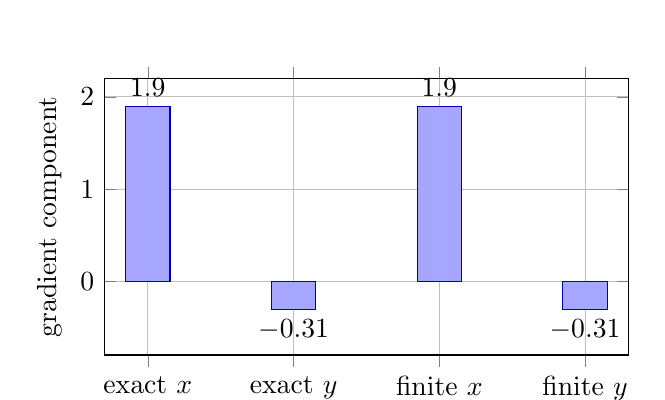
\begin{tikzpicture}
\begin{axis}[
  ybar,
  width=0.68\textwidth,
  height=0.42\textwidth,
  symbolic x coords={exact $x$,exact $y$,finite $x$,finite $y$},
  xtick=data,
  ymin=-0.8,ymax=2.2,
  ylabel={gradient component},
  nodes near coords,
  nodes near coords align={vertical},
  grid=both,
  bar width=16pt,
]
\addplot[fill=blue!35,draw=blue!70!black] coordinates {(exact $x$,1.90) (exact $y$,-0.31) (finite $x$,1.90) (finite $y$,-0.31)};
\end{axis}
\end{tikzpicture}
\caption{Finite differences approximate the gradient when symbolic derivatives are unavailable.}
\end{figure}

\section{Common mistakes}

\begin{warningbox}[Frequent errors]
\begin{enumerate}
  \item Forgetting to normalize the direction vector. Directional derivative formulas require a unit vector.
  \item Assuming every critical point is an extremum. Saddle points are common in several variables.
  \item Using the second derivative test when $D=0$. The test gives no conclusion in this case.
  \item Ignoring the boundary. Absolute extrema on closed regions may occur on the boundary.
  \item Choosing a learning rate blindly. In gradient descent, too large a learning rate may cause divergence or oscillation.
  \item Confusing local and global behavior. A local minimum may not be the absolute minimum.
\end{enumerate}
\end{warningbox}

\section{Chapter summary}

The directional derivative measures the rate of change of a function in a chosen direction:
\[
D_u f=\grad f\cdot u.
\]
The gradient is the direction of steepest increase, and the negative gradient is the direction of steepest decrease. Critical points occur where the gradient vanishes or where derivatives fail to exist. The Hessian matrix provides second derivative information, and the determinant
\[
D=f_{xx}f_{yy}-f_{xy}^2
\]
classifies nondegenerate critical points in two variables.

For absolute extrema on closed bounded regions, critical points are not enough: the boundary must also be checked. In computational settings, gradient descent and Newton's method turn these ideas into algorithms for fitting models and minimizing loss functions.

\section{Exercises}

\subsection*{Conceptual questions}
\begin{enumerate}
  \item Explain in words what $D_u f(a,b)$ measures.
  \item Why must $u$ be a unit vector in the definition of directional derivative?
  \item Explain why the gradient points perpendicular to level curves.
  \item What is the difference between a critical point and a local minimum?
  \item Why does $D<0$ in the second derivative test indicate a saddle point?
  \item Why must boundary points be checked when finding absolute extrema?
  \item Explain the relationship between gradient descent and steepest descent.
  \item Why can Newton's method fail near a saddle point?
\end{enumerate}

\subsection*{Computational practice}
\begin{enumerate}
  \item Let $f(x,y)=x^2+xy+y^2$. Compute $D_u f(1,2)$ in the direction of $v=\langle 3,4\rangle$.
  \item Let $f(x,y)=e^{xy}+y^3$. Find the direction of fastest increase at $(1,0)$ and the maximum rate of increase.
  \item Let $f(x,y,z)=x^2y+yz^2$. Compute the directional derivative at $(1,2,-1)$ in the direction of $v=\langle 1,0,2\rangle$.
  \item Find and classify the critical points of $f(x,y)=x^2+y^2-6x+4y+20$.
  \item Find and classify the critical points of $f(x,y)=x^2-y^2+4x+2y$.
  \item Find and classify the critical points of $f(x,y)=x^3+y^3-6xy$.
  \item Find and classify the critical points of $f(x,y)=x^4+y^4-4xy$.
  \item Find the absolute maximum and minimum of $f(x,y)=x+y$ on the square $0\le x\le 1$, $0\le y\le 2$.
  \item Find the absolute maximum and minimum of $f(x,y)=x^2+y^2-2x$ on the disk $x^2+y^2\le 4$.
  \item Run gradient descent on $L(x,y)=(x-3)^2+4(y+1)^2$ from $(0,0)$ with several learning rates. Describe what changes.
\end{enumerate}

\subsection*{Applied and data-oriented problems}
\begin{enumerate}
  \item A model has loss $L(w_1,w_2)=4(w_1-2)^2+(w_2+1)^2+w_1w_2$. Find the critical point and classify it.
  \item For least squares with data $(x_i,y_i)$, derive the gradient of $L(\beta_0,\beta_1)=\sum_i[y_i-(\beta_0+\beta_1x_i)]^2$.
  \item Suppose a log-likelihood $\ell(\theta_1,\theta_2)$ has Hessian negative definite at a critical point. What does that tell you about the likelihood locally?
  \item A neural-network training loss has a point where $\grad L=0$ but the Hessian has both positive and negative eigenvalues. What kind of point is this?
  \item Write a function that approximates the gradient of a function $f:\R^n\to\R$ using central differences.
\end{enumerate}

\section{Python lab}

The Chapter 11 Python lab asks you to:
\begin{enumerate}
  \item compute directional derivatives numerically and analytically;
  \item visualize gradient vectors on contour maps;
  \item classify critical points using the Hessian determinant;
  \item implement gradient descent on quadratic and least-squares losses;
  \item compare gradient descent with a damped Newton method.
\end{enumerate}

\section{Looking ahead}

This chapter focused on unconstrained optimization and boundary checks. The next chapter develops constrained optimization systematically. The key geometric idea will be that, at a constrained optimum, the gradient of the objective is parallel to the gradient of the constraint.

\end{document}
